\documentclass[12pt,a4paper,oneside]{report} %class

% encode foregin characters
\usepackage[T1]{fontenc}

% hungarian language
\PassOptionsToPackage{defaults=hu-min,classmod=unchanged}{magyar.ldf}
\usepackage{t1enc}
\usepackage[magyar]{babel}
\selectlanguage{magyar}
\usepackage[utf8]{inputenc}

\usepackage{csquotes}

\usepackage{paralist}

%\usepackage{float}
%\usepackage{tabularx}
%\usepackage[table]{xcolor}

% images 
\usepackage{graphicx}
\graphicspath{ {./images/} }

% set margins
\addtolength{\oddsidemargin}{-1.2cm}
\addtolength{\evensidemargin}{-1.2cm}
\addtolength{\textwidth}{2.4cm}
\addtolength{\topmargin}{-1.5cm}
\addtolength{\textheight}{3cm}

% set TOC depth
\setcounter{tocdepth}{4}

% remove red color for hyperref in TOC
\usepackage[unicode]{hyperref}
\hypersetup{
	colorlinks,
	citecolor=black,
	filecolor=black,
	linkcolor=black,
	urlcolor=black
}


% add bibtex
\usepackage[backend=biber]{biblatex}
\BiblatexHungarianWarningOff
\addbibresource{./mainbibliography.bib}



%top matter
\title{%
	
\includegraphics[scale=0.1]{logo_oe}\\
	ÓBUDAI EGYETEM\\
	Neumann János Informatikai kar\\
	Mérnök informatikus BSc\\
	\vfill
	\large \textbf{Vizuális, interaktív programozás oktató rendszer moduláris megvalósítása\\}
	\large Projektmunka dokumentáció
	\vfill
}
\author{Ráncsik Áron}
\date{\today}

\begin{document}

\pagenumbering{Alph}
\begin{titlepage}
\maketitle
\thispagestyle{empty}
\end{titlepage}
\pagenumbering{arabic}

\pagenumbering{Alph}
\begin{abstract}
	\thispagestyle{empty}
	Your abstract goes here...
	...
\end{abstract}
\pagenumbering{arabic}

\tableofcontents

% Introductory chapters
\chapter{Bevezetés}
\par 
Az oktatásban manapság elterjedt\cite{riar2020game} gyakorlat az oktatott anyag játékos megfogalmazása, idegen szóval a \cite{Deterding2011}\textit{gamification}. A módszer lényege, hogy a megtanítani kívánt ismeretet egyszerű, nyers forma helyett, játékos formában tesszük emészthetővé a tanulók számára. Dolgozatomban szeretném a tanulni vágyok elé tárni a programozást, olyan formában, hogy az ne okozzon nehézséget, illetve a tanulás emléke inkább egy élmény legyen, egy unalmas óra helyett.
\par Az alábbi célokat tűztem ki. Legyen lehetőség kézvezérléssel végezni a programozást. Programozás egyik motivációja , hogy a felhasználók által készített különböző programkódok, ágensek egymás ellen tudjanak versenyezni. A megmérettetést akár már létező, ismert számítógépes játékokhoz csatlakozva, vagy saját egyedi játékban tehetik meg. Egy másik tervezett funkció, hogy az írt kódok összecsapását pedig kiterjesztett valóságon keresztül szeretném követni. További cél, hogy legyen lehetőség az egyetemen elérhető DaVinci roboton is könnyen magas-szintű programkódot futtatni.
\par Röviden összefoglalva, a következő irodalomkutatást készítettem a fent megfogalmazott célokra. Első lépésként,  a kitűzött célokat  megvalósítsa érdekében, a \ref{vizuprogkor} részben a vizuális programozási környezet elkészítésének lehetőségeit részletezem, mely abban segít, hogy egy konkrét programozási nyelv tanulásának kezdeti nehézségein átugorva vizuális eszközökkel teszi elérhetővé a programozást, akár laikusok számára is. A \nameref{modtan} szekció \ref{davinci} részben azt vizsgálom, milyen lehetőségek vannak a Da Vinci robot egyszerű maga-szintű programozására. A \ref{kitvalo} szekcióban a kiterjesztett valóság megvalósításának lehetőségeit részletezem. A \nameref{modtan} utolsó szekciójában \ref{kezvez} a kézvezérlés funkció megvalósításához szükséges ismereteket igyekszem analizálni. 
\par 

%\section{Algoritmus elmélet}
%Az algoritmus definiálása nehéz feladat, erre nem vállalkoznék, az kijelenthető, hogy azokat a feladatokat lehet algoritmizálni melyek működése Turing gép segítségével megvalósítható.  

\chapter{Módszertan}
\label{modtan}
Itt a korában megfogalmazott célok elérése érdekében végzett kutatómunkát részletezem.
\section{Vizuális programozási környezet}
\subsection{Alternatív megoldások vizuális programozásra}
\label{vizuprogkor}
Mivel a dolgozatban részben vizuális  programozást  is szeretnék biztosítani, ezért megvizsgálom milyen konkurens megoldások léteznek erre a célra. Az alábbiakban bemutatok és elemzek több kutatást, korábbi kész alkalmazásokat és programkönyvtárakat melyek mindegyike a vizuális blokk alapú programozást nyújtja.
\paragraph{Scratch} 
\label{scratch}
Nagyon népszerű, oktatásban méltán közkedvelten használt teljes környezet \cite{maloney2010scratch, resnick2009scratch, ScratchUrl2019Jan}, mely vizuális programozást tesz lehetővé. Az alapvető célja olyan média alkalmazások mint pl.: animáció, köszöntések, történet mesélés, zeneklip elkészítésének folyamata közben megtanítani a programozást. Az egyedüli, intuitív tanulás is előnyben részesíti. Főleg kisebb 8-16 éves korosztály számára készült. 
\par Az elkészült program alapértelmezetten egy saját ``{színpad}'' környezetben futtatható. Esemény vezérelt programozást is lehetővé tesz, ebben az esetben az egyszerre fellépő konkurens utasítások között esetleges versenyhelyzetet kezeli, de nem minden esetben úgy ahogy azt elsőre a használó gondolná.  A programból \textit{broadcast} utasításokkal, saját parancsok, szkriptek végrehajtása lehetséges. A \textit{broadcast} utasítássokkal lehetséges a külvilággal történő kommunikáció is, de körülményes. Kiegészítőkkel bővíthető, de így sem nem lehet az alap működésre kiható szignifikáns módosításokat végrehajtani.
\subparagraph{Előnyei} 
\begin{compactitem}
	\item Szabadon elérhető, nyílt forráskódú.
	\item Kész megoldásról beszélve, sokkal kevesebb munka segítségével lehet használni.
	\item Egyedi működés \textit{broadcast} utasításokkal lehetséges.
	\item Az alap környezet többnyire magas szintű előre definiált utasításokban gazdag pl.: animációk
	\item Kezdők számára is egyszerűen érthető felület.
	\item Tapasztalatok alapján nagyon ismert az általános iskolások körében.
	\item Érthető, naprakész dokumentáció áll rendelkezésre
\end{compactitem}
\subparagraph{Hátrányai} 
\begin{compactitem}
	\item A \textit{broadcast} utasításon kívül máshogy nem megoldható egyedi utasítás létrehozása.
	\item Az elkészült program csak a saját környezetén belül futtatható, nem lehetséges egyedi környezetben futtatni.
	\item Az elkészült program egyszerűen nem alakítható valódi programkóddá. (Van harmadik féltől származó kész megoldás)
	\item Monolitikus, bővítésre nézve többnyire zárt rendszer.
	\item Ugyan van webes felület, de saját oldalba nem ágyazható.
\end{compactitem}

\paragraph{Snap} \label{snap}Új, még kevésbé  ismert, teljes megoldás \cite{harvey2013snap}, segítségével vizuálisan van lehetőségünk programozni. A \nameref{scratch}-el szemben több szabadságot biztosít a személyre szabhatóság tekintetében. Sokkal bonyolultabb problémák megoldására is alkalmas, az objektum orientált paradigmát is támogatja. A környezet kevésbé kezdő barát. \textit{Url} utasításokkal webes  csatlakozó felületen keresztül tud fogadó és küldőként is könnyen kommunikálni a külvilággal. A felhő alapú gépi tanulás szolgáltatásokhoz csatlakoztatva akár ``AI'' fejlesztésre is alkalmas \cite{kahn2018ai}. A párhuzamos ciklusokat időosztásos módszerrel futtatja párhuzamosan ``yield'' utasítások segítségével, de erre is igaz. hogy mindezt igyekszik elrejteni a felhasználók elől és nem igényel különösebb beavatkozást az alapvető működéshez hozzá lehet szokni.
\subparagraph{Előnyei} 
\begin{compactitem}
	\item Szabadon elérhető, nyílt forráskódú.
	\item Kész megoldásról beszélve, sokkal kevesebb munka segítségével lehet használni.
	\item Egyedi működés \textit{url} utasításokkal lehetséges. Sokkal kényelmesebben mint \nameref{scratch} esetén.
	\item Az alap környezet előre definiált utasításokban gazdag pl.: \textit{sprite}-ok vezérlése.
	\item Bonyolultabb problémák megoldására is alkalmas.
	\item Érthető, naprakész dokumentáció áll rendelkezésre
	\item Van webes felülete, de saját oldalba nem ágyazható.
	\item Egyedi blokkok létrehozását támogatja.
	\item Objektum orientált paradigmát támogatja
\end{compactitem}
\subparagraph{Hátrányai} 
\begin{compactitem}
	\item Az elkészült program csak a saját környezetén belül futtatható, nem lehetséges egyedi környezetben futtatni.
	\item Az elkészült program nem alakítható valódi programkóddá.
	\item Nem biztosít felhasználható könyvárat, csak a projekt forrását felhasználva lehet egyedi alkalmazásokban használni.
	\item Jelenleg (\date{\today}) béta állapotban van.
	\item Monolitikus, bővítésre nézve többnyire zárt rendszer.
	\item A objektum orientáltság különböző megkötésekkel érhető el.
\end{compactitem}

\paragraph{GP} Általános célú blokk alapú \cite{ohshima2015module} \cite{monig2015blocks} programozási nyelv. Egy valódi programozási nyelv mely blokk és kód alapú programozási lehetőséggel is rendelkezik.  Sok alacsony szintű funkciók érhetőek el benne. Sokkal közelebb áll a valóságos programozáshoz a korábban említett lehetőségekhez képest, rendelkezik webes felülettel és a külvilággal internetes \textit{get}, \textit{put} utasítás lehetséges a kommunikáció egyedi rendszerekkel. Támogatja az objektum orientált paradigmát. Tartalmaz bonyolultabb adatszerkezeteket is.
\subparagraph{Előnyei} 
\begin{compactitem}
	\item Kész megoldásról beszélve, sokkal kevesebb munka segítségével lehet használni.
	\item Egyedi működés \textit{get, put} utasításokkal lehetséges. \newline Sokkal kényelmesebben mint \nameref{scratch} esetén.
	\item Az alap környezet többnyire alacsony szintű előre definiált utasításokban gazdag pl.: \textit{set pixel} utasítás blokk.
	\item Bonyolultabb problémák megoldására is alkalmas.
	\item Moduláris módon készült.
	\item Érthető, naprakész dokumentáció áll rendelkezésre.
\end{compactitem}
\subparagraph{Hátrányai} 
\begin{compactitem}
	\item Az elkészült program csak a saját környezeten belül futtatható, nem lehetséges saját környezetben futtatni.
	\item Az elkészült program nem alakítható valódi programkóddá.
	\item Ugyan van webes felület, de saját oldalba nem ágyazható.
\end{compactitem}

\paragraph{Alice} Interaktív 3D Animációs környezet \cite{cooper2000alice}. Az idézett kutatás által megfogalmazottan a  célja egy 3D-s környezet interaktív fejlesztése melyben szabadon lehet felfedezni az elkészült alkotást. Főleg szkript alapú prototípus fejlesztő környezet. 
\subparagraph{Előnyei} 
\begin{compactitem}
	\item Kész munka elvileg kevesebb munka lehet átalakítani, felhasználni
	\item Adott 3D környezet
	\item Esemény vezérelt programozás tanítására is alkalmas
\end{compactitem}
\subparagraph{Hátrányai} 
\begin{compactitem}
	\item Az elkészült program csak a saját környezeten belül futtatható, nem lehetséges saját környezetben futtatni.
	\item Nem vizuális egy sajátos egyedi szkriptnyelvvel rendelkezik.
	\item Az elkészült program nem alakítható valódi programkóddá.
	\item Nincs webes felülete, futtatható állományok telepítését igényli.
	\item Kissé régi, idejét múlt, már kevésbé támogatott.
\end{compactitem}

\paragraph{Egyéb kész megoldások}
A fenti részben az általam, a dolgozatommal legjobban összehasonlítható szempontok alapján fontosnak tartott kész megoldásokat mutattam be. Természetesen rengeteg egyéb kész alkalmazás létezik mely vizuális programozási lehetőséget biztosít. Felsorolás szintjén itt leírok pár szerintem említésre méltó alkalmazást. 
\begin{compactitem}
	\item Game Maker \cite{jenson2016exploring} 2D játék készítő, vizuális és saját szkriptnyelvvel is rendelkezik. A teljes verzió pénzbe kerül.
	\item Stencyl \cite{liu2014making} 2D Játék készítő alkalmazás melyben vizuálisan lehet programozni.
\end{compactitem}
A továbbiakban kész alkalmazások helyett, vizuális programozásra készült programkönyvtárak bemutatásával fogom folytatni az választható megoldások listáját.  
\paragraph{Blockly}
\label{blocly}
Google által fejlesztett, vizuális programozást támogató program könyvtár \cite{BlocklyUrl2020Feb} \cite{pasternak2017tips}. A vizuális megjelenésért felelős, nem egy programozási nyelv, csak egy vizuális leíró nyelv, mely könnyedén exportálható vallós programozási kóddá. Több létező programozási nyelv kódot lehet a vizuális környezetből generálni, többek között: Javascript, Python, Lua, Dart nyelvű kódokat is. A Blockly könyvtárat sok kész alkalmazás használja a saját egyedi vizuális környezetének megvalósítására.
Például a korábban említett \nameref{scratch}, \nameref{snap} is használja vizuális könyvtárként, de az ezután részletezett \nameref{pxt} környezet is Blockly-t használ a vizuális megjelenítésre.
\subparagraph{Előnyei} 
\begin{compactitem}
	\item Szabadon elérhető, nyílt forráskódú.
	\item Kezdők számára is egyszerűen érthető felület.
	\item Érthető, naprakész dokumentáció áll rendelkezésre.
	\item Program könyvtár, könnyen bővíthető egyedi utasításokkal
	\item A program futtatási környezetére nincs megkötés.
	\item Nemzetközi. Több mint 40 (köztük magyar) nyelven elérhető.
	\item Bármilyen futtatási környezetbe könnyen integrálható.
	\item Rengeteg programkód generálható.
\end{compactitem}
\subparagraph{Hátrányai} 
\begin{compactitem}
	\item Csak egy vizuális programozást támogató  ``drag \& dropp'' programkönyvtár.
	\item Viszonylag régi technológiákkal készült, nehézkes modern környezetben használni.
\end{compactitem}

\paragraph{MakeCode (PXT)}
\label{pxt}
Microsoft által fejlesztett, összetett, vizuális programozói környezet támogató, nyílt forráskódú programkönyvtár \cite{seneviratne2019makecode}. A \nameref{blocly} könyvtárat felhasználja a blokk alapú vizuális programozás biztosítására. A blokk alapú programozáson túl biztosít lehetőséget a szöveges programozásra is, egy beépített weboldalon futamítható fejlesztő környezetben. Abban különbözik a korábban alternatív lehetőségektől, hogy egyben nyújt egy teljes fejlesztő környezetet, amihez könnyen hozzá lehet csatolni egy saját \textit{target} modult egyedi utasításokkal. \cite{devine2018makecode} Kutatás részletesen bemutatja, hogyan lehet használni beágyazott rendszerekhez. A fejlesztő környezethez alacsony szintű mikrokontrollerhez való fordítót csatlakoztatva.
\subparagraph{Előnyei} 
\begin{compactitem}
	\item Szabadon elérhető, nyílt forráskódú.
	\item Kezdők számára is egyszerűen érthető felület.
	\item Érthető, naprakész dokumentáció áll rendelkezésre.
	\item Program könyvtár, könnyen bővíthető egyedi utasításokkal
	\item A program futtatási környezetére nincs erős megkötés.
\end{compactitem}
\subparagraph{Hátrányai} 
\begin{compactitem}
	\item Integrálása korlátozott, alkalmazkodni kell a felépítéséhez, ettől eltérni nem lehetséges könnyen.
	\item Béta verzióban van a fejlesztés.
\end{compactitem}

\subsubsection{Választott vizuális programozási környezet}
Kipróbáltam, teszteltem a felsorolt megoldásokat továbbá a korábbi elemzés összevetése  után a Blockly környezet használata mellet döntöttem.
A dolgozat igényeit nem lehet kész megoldásokkal pl. \nameref{scratch}, \nameref{snap} stb. kielégíteni, mert túlságosan zárt működésük nem teszik lehetővé, hogy egyedei játékhoz lehessen programozni ezekben az alkalmazásokban.
A Blockly kellőképpen módosítható és könnyen beilleszthető, vizuális programozást biztosító programkönyvtár, mely megfelel a feladat részéről támasztott elvárásoknak.


\section{Da Vinci}
Az célok között szerepelt a Da Vinci robot egyszerű vezérlése. Az elkövetkező részben, igyekszem körbejárni a lehetőségeket és azok előnyeit hátrányait. Az egyetemen egy 2010-es első generációs da Vinci classic rendszerhez van lehetőség hozzáférni. Ezért ehhez készült az alkalmazás. A továbbiakban mindig erről a modellről lesz szó.
\paragraph{Robot Operating System}
Annak érdekében, hogy a fejlesztés során, ne kelljen folyamatosan a fizikai Da Vinci rendszerhez hozzáférnem, egy olyan környezetre van szükségem ami képes biztosítani a Da Vinci robotot virtuálisan. Ugyan sok rendszer elérhető csak felsorolás szintjén néhány mely robot vezérlő környezetet biztosít azonban az egyik legkorábbi és legnépszerűbb lehetőség a Robot Operating System \cite{quigley2009ros} továbbiakban csak ROS. Dolgozatomban több szempont miatt is a legjobb választásnak a ROS rendszert bizonyult. Attól a hátrányától eltekintve, hogy nem multiplatform azaz csak Ubuntu GNU/Linux és annak is csak bizonyos verzióihoz elérhető rengeteg előnnyel rendelkezik. Sok robot vezérléssel kapcsolatos alapfunkciót tartalmaz, amit így nem kell újból megírni, biztosít egy jól elszeparált keretet külön a kommunikációra és az üzleti logikára.
\subparagraph{Előnyei} 
\begin{compactitem}
	\item Szabadon elérhető, nyílt forráskódú
	\item Kiforrót
	\item Népszerű
	\item Moduláris
	\item Kutatási célokhoz megfelelő
	\item Érthető, naprakész, jó dokumentáció áll rendelkezésre
\end{compactitem}
\subparagraph{Hátrányai} 
\begin{compactitem}
	\item Nem multiplatform, csak Ubuntu GNU/Linux és annak is csak bizonyos verzióihoz elérhető
\end{compactitem}

\subsubsection{Da Vinci Research Kit}
\label{davinci}
A Da Vinci Research Kit \cite{kazanzides2014open} továbbiakban DVRK egy nyílt forráskódú rendszer ami lehetővé teszi a Da Vinci robot karok programozását. A ROS rendszerhez kapcsolódik, könnyen lehetséges az utasításait használni egy ROS modult  node-ot biztosít használatra.  A célkitűzéseimhez képest viszonylag alacsony-szintű Da Vinci robot kar vezérlő utasítások kiadására alkalmas.

\subsubsection{iRob Surgical
Subtask Automation Framework}
\label{irob}
Nagy Tamás és Haidegger Tamas által fejlesztett keretrendszer  \cite{irobsaf2019}.
Alapvetően arra a célra készült, hogy részleges automatizáció segítségével levegye a sebészekről a kognitív terhelést. Részfolyamatok automatizálását teszi lehetővé a keretrendszer. A ROS rendszerben elérhető node-okat biztosít, a DVRK rendszerre épül. Felépít egy hierarchikus node rendszert melynek a legmagasabb szintjén magas-szintű utasítások kiadása lehetséges. Számomra a céloknak tökéletesen megfelelő.
\subparagraph{Előnyei} 
\begin{compactitem}
	\item Szabadon elérhető, nyílt forráskódú
	\item Moduláris
	\item Kutatási célokhoz megfelelő
	\item Érthető, naprakész, jó dokumentáció áll rendelkezésre
\end{compactitem}
\subparagraph{Hátrányai} 
\begin{compactitem}
	\item Jelenleg fejlesztés alatt áll.
\end{compactitem}


\section{Kiterjesztett valóság}
\label{kitvalo}
A \cite{azuma2001recent} kutatásból idézve  kiterjesztett valóságot a következő módon definiálhatjuk: Kiterjesztett valóság az a rendszer, ami a következőket teljesíti:
\begin{compactitem}
	\item Kombinálja a valós és virtuális objektumokat a valós környezetben.
	\item Azonnal fut, és valós időben.
	\item Egymáshoz rögzíti (igazítja) %a valós és virtuális objektumokat.
\end{compactitem}
Virtuális objektumokat szeretnénk elhelyezni a kamera képen úgy, hogy azok mozgása a kamera 3D mozgásához igazodjon. 
 \par Több létező megoldás van kiterjesztett valóság elkészítéséhez, ezen megoldások összehasonlításáról lesz itt szó.

\section{Kézvezérlés}
\label{kezvez}

\section{Gépi látás}
\section{Kamera mozgás becslés}
\subsection{Markerek keresése}


\chapter{Megvalósítás}
\section{Da Vinci webes elérhetősége}
Először meg kellet ismerkednem a korábban részletezett \ref{irob}, \cite{irobsaf2019} keretrendszettszer és ROS architektúra használatával. Az irob\_saf keretrendszer működését a \ref{fig:irob} ábra szemlélteti.
\begin{figure}
	\label{fig:irob}
\begin{center}
	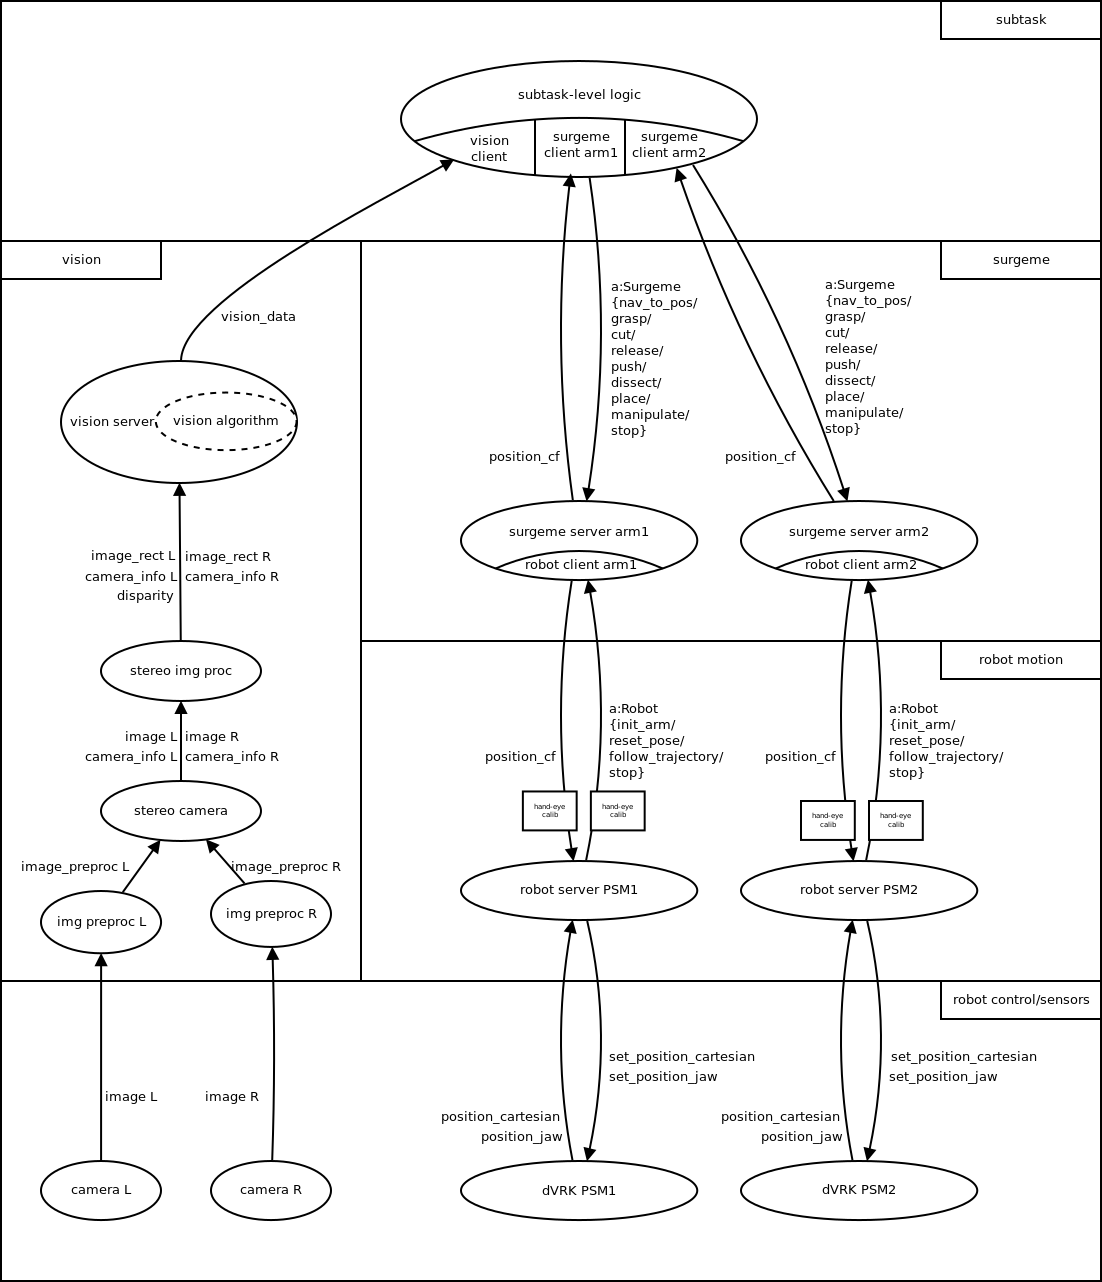
\includegraphics[width=14cm]{irobArch}
	\caption{A irob\_saf keretrendszer működését szemléltei}
\end{center}
\end{figure}
\newpage
\chapter*{Irodalomjegyzék}
\addcontentsline{toc}{chapter}{Irodalomjegyzék}  
\printbibliography[heading=none]
\newpage
\listoffigures
\addcontentsline{toc}{chapter}{Ábrák jegyzéke}


\end{document}